\documentclass[12pt,a4paper]{report}
\usepackage[utf8]{inputenc}
\usepackage[T1]{fontenc}
\usepackage{fontspec}
\usepackage[polish]{babel}
\usepackage{amsmath}
\usepackage{graphicx}
\usepackage[table,xcdraw]{xcolor}
\usepackage{hhline}
\usepackage{placeins}
\usepackage[margin=0.6in]{geometry}
\usepackage{appendix}
\usepackage{colortbl}
\usepackage{physics}
\usepackage{float}
\usepackage{datetime}
\usepackage{makeidx}
\usepackage{hyperref}

\title{Mechanika Kwantowa R 2021/2022}
\author{Kacper Cybiński}
% \newdate{date}{28}{01}{2022}
% \date{\displaydate{date}}
\date{\today}
\makeindex
\setlength\parindent{0pt}

\addto\captionspolish{\renewcommand{\chaptername}{Lecture}}

\newcommand{\ind}[1]{{\color{blue} #1\index{#1}}}

\newcommand{\subind}[2]{{\color{blue} #1\index{#2}}}

\newcommand{\com}[1]{{\color{red} #1}}

\newcommand{\link}[2]{{\color{cyan} \href{#1}{#2}}}

\newcommand{\uwaga}[1]{{\color{violet} Uwaga:} #1}

\newcommand{\phys}{\stackrel{\text{F}}{\equiv}}

\newcommand{\E}{\mathcal{E}}

\newcommand{\R}{\mathcal{R}}

\newcommand{\T}{\mathcal{T}}

\newcommand{\HS}{\mathcal{H}}

\newcommand{\CS}{\mathcal{C}}

\renewcommand{\emph}{\textbf}

\newenvironment{lecture}[1][]{\par\medskip
   \noindent\chapter \rmfamily}{\medskip}
   
\newenvironment{emph_box}[1]
    {\begin{center}
    \begin{tabular}{|p{0.9\textwidth}|}
    \hline
    \begin{center} \textbf{#1} \end{center}\\[1ex]
    }
    { 
    \\\\\hline
    \end{tabular} 
    \end{center}
    }

\begin{document}

\maketitle

\chapter*{Organizacja wykładu}
\begin{enumerate}
    \item Dwa kolokwia - po 30 pkt
    \item Egzamin - 40 pkt
\end{enumerate}
Łącznie 100 pkt, progi punktowe:
\[45-55 = 3, 55-65 = 3.5, 65-75=4, 75-85=4.5, 85-95 = 5, 95-100=5!\]

Egzamin ustny (zmiana oceny co najwyżej o 0.5)

Serie domowe dobrowolne (ale na pewno pomogą napisać dobrze kolokwia!)

{\color{blue} \link{https://kampus-student2.ckc.uw.edu.pl/course/view.php?id=9707}{Strona wykładu}}


Polecane podręczniki:
\begin{itemize}
    \item L. Schiff \textit{Mechanika Kwantowa (obszerna)}
    \item R. Liboff \textit{Wprowadzenie do Mechaniki Kwantowej} \textit{(mniej obszerna)}
    \item L. Susskind \textit{Quantum Mechanics (Do ogarnięcia koncepcyjnego)}
\end{itemize}

\begin{lecture}
    \section{Krótka historia fizyki}
    \begin{itemize}
        \item {\bf Arystoteles} - Jeden absolutny układ odniesienia, więc nie ma sensu pojęcie \textit{obserwatora}
        \item {\bf Newton} - Ciała, a więc i układy odniesienia (obserwatorzy inercjalni) są liczne, oraz mogą się poruszać między sobą. Siła, czas, przestrzeń są wciąż pojęciami absolutnymi.
        \item {\bf Teoria względności} - Ruch, czas, przestrzeń, masa są zależne od obserwatora. Obserwator nie musi być inercjalny. Mówimy o {\it Uoperacyjnieniu pojęć zasadniczych}.
        \item {\bf Teoria Kwantowa} - Okazuje się, że cały zestaw wielkości fizycznych służących do opisu świata zależy od tego jaki jest kontekst pomiarowy, tj. od relacji obserwatora z innymi elementami otaczającego go świata. {\it Czyli po raz pierwszy uwzględniamy fakt, że opisujemy wszechświat w którym sami istniejemy, czyli opisujemy ten układ {\bf od środka}}.
    \end{itemize}
    \link{http://studenci.fuw.edu.pl/~kc427902/Prezentacje_Kwanty/HisotriaFIzykiWitkacy.pdf}{Prezentacja o historii fizyki wg Witkacego}
    
    
    \section{Hipoteza Kwantu}
    Co doprowadziło do wniosków, że energię trzeba skwantować?
    \subsection{Ciało Doskonale Czarne}
    Paradoks polegał na tym, że z ciała doskonale czarnego powinniśmy mieć zabójcze promieniowanie gamma itp, a go nie było IRL. And here comes the {\it Max Planck}.\\
    Planck zapostulował, że przekaz energii odbywa się za pomocą całkowitych wartośći (\ind{Kwant Energii})
    Zdefiniował to jako:
    \begin{equation}
        E = h \cdot \nu = \hbar \cdot \omega
        \label{lec_1:eq:E_planck}
    \end{equation}
    \[\hbar = \frac{h}{2 \pi}, \omega = 2 \pi \nu\]
    gdzie h - \ind{stała Plancka}, $h = 6.2626070150 \cdot 10^{-34} J\cdot s$, $\nu$ - częstotliwość promieniowania 
    \begin{figure}[!ht]
        \centering
        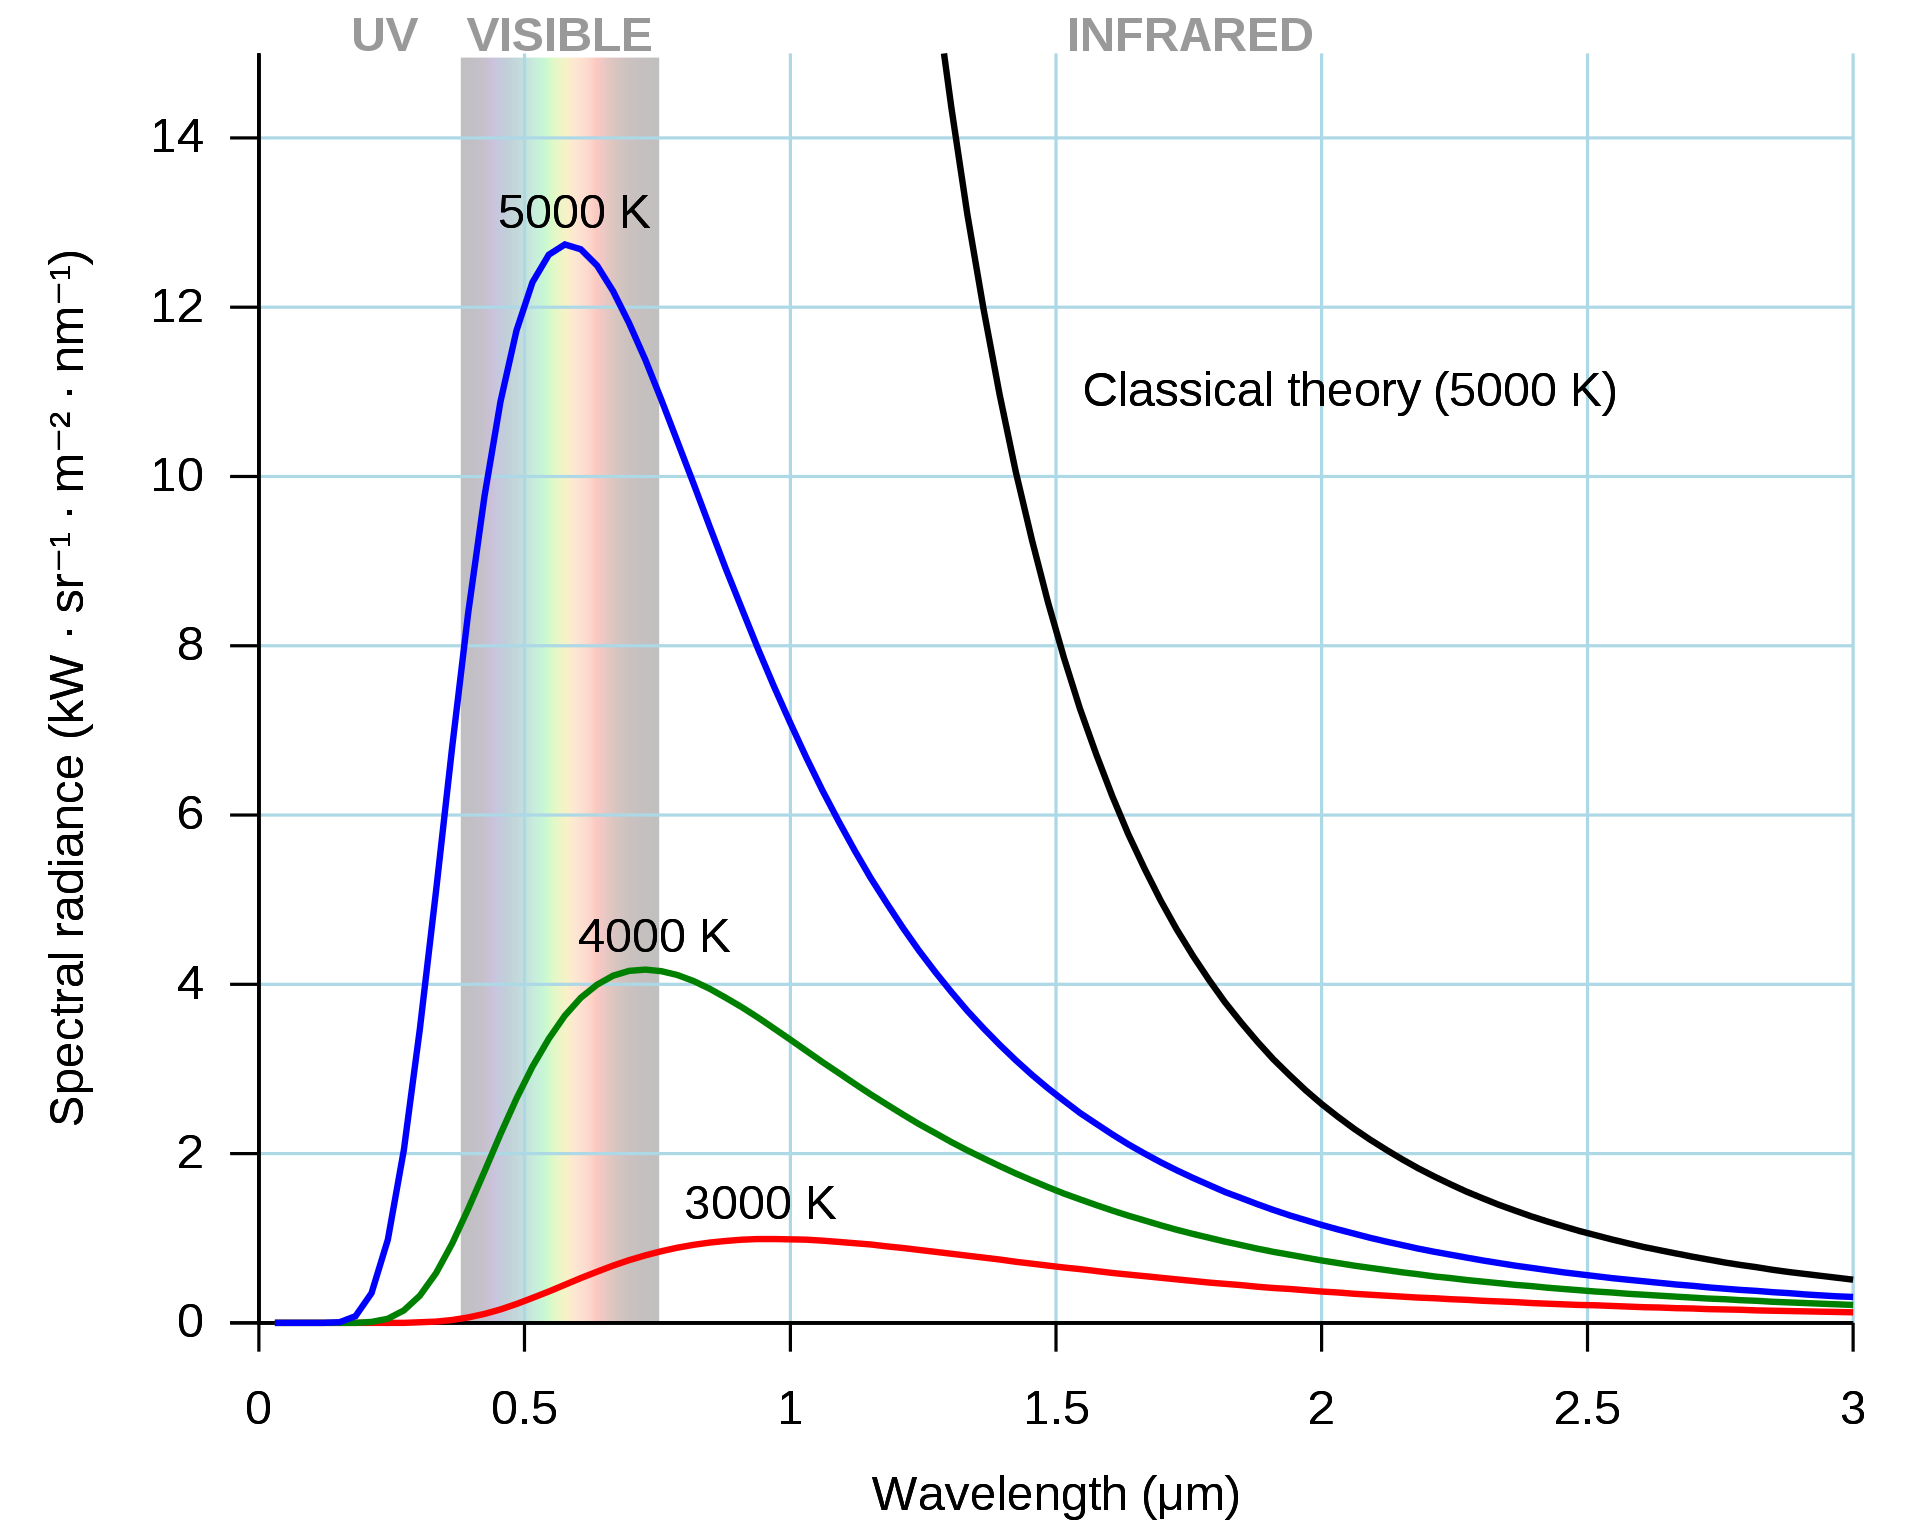
\includegraphics[width=\linewidth]{Wyk_1_Rys_5.png}
        \caption{Wykres promieniowania ciała doskonale czarnego}
        \label{lec_1:fig:cialo_doskonale_czarne}
    \end{figure}
    
    \begin{figure}[!ht]
        \centering
        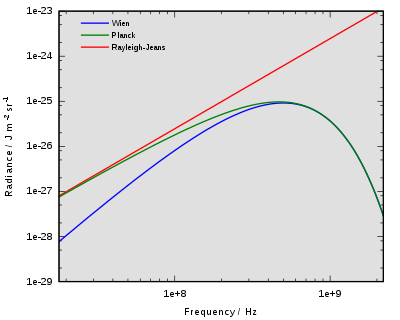
\includegraphics[width=\linewidth]{Wyk_1_Rys_6.png}
        \caption{Porównanie hipotezy Plancka z prawem Rayleigha-Jeansa i rozkładem Wiena. Further reading o 'Katastrofie w nadfiolecie'  na \link{https://pl.wikipedia.org/wiki/Ciało_doskonale_czarne}{Wikipedii o ciele doskonale czarnym}}
        \label{lec_1:fig:cialo_doskonale_czarne_porownanie}
    \end{figure}
    
    \subsection{Efekt Fotoelektryczny}
    \subsection{Analiza pól EM}
    Analiza pól $\E$ i B w odniesieniu do sześcianu z przewodnika prowadzi do wniosku, że energia "porcji promieniowania" transformuje się jak 
    \[\frac{\E'}{\E} = \frac{\sqrt{1 - \frac{u}{c}}}{\sqrt{1 + \frac{u}{c}}}\]
    gdzie $u$ - promieniowanie.
    Transformuje się to analogicznie do częstotliwości w efekcie Dopplera $\implies E \sim \nu$
    \\
    Rozkład energii będzie nam opisywać \ind{Rozkład Boltzmanna}, czyli rozkład prawdopodobieństwa zaobserwowania stanu Energetycznego, dany wzorem:
    \[p(E_i) \sim e^{-\frac{E_i}{k T}}\]
    co w przypadku rozkładu ciągłego daje nam zasadę ekwipartycji, ale dla dużych wartości energii się rozbiega z doświadczenie.
    
    \section{Skutki skwantowania energii}
    Przede wszystkim skutkiem jest \ind{indeterminizm}.\\
    
    \begin{figure}[!ht]
        \centering
        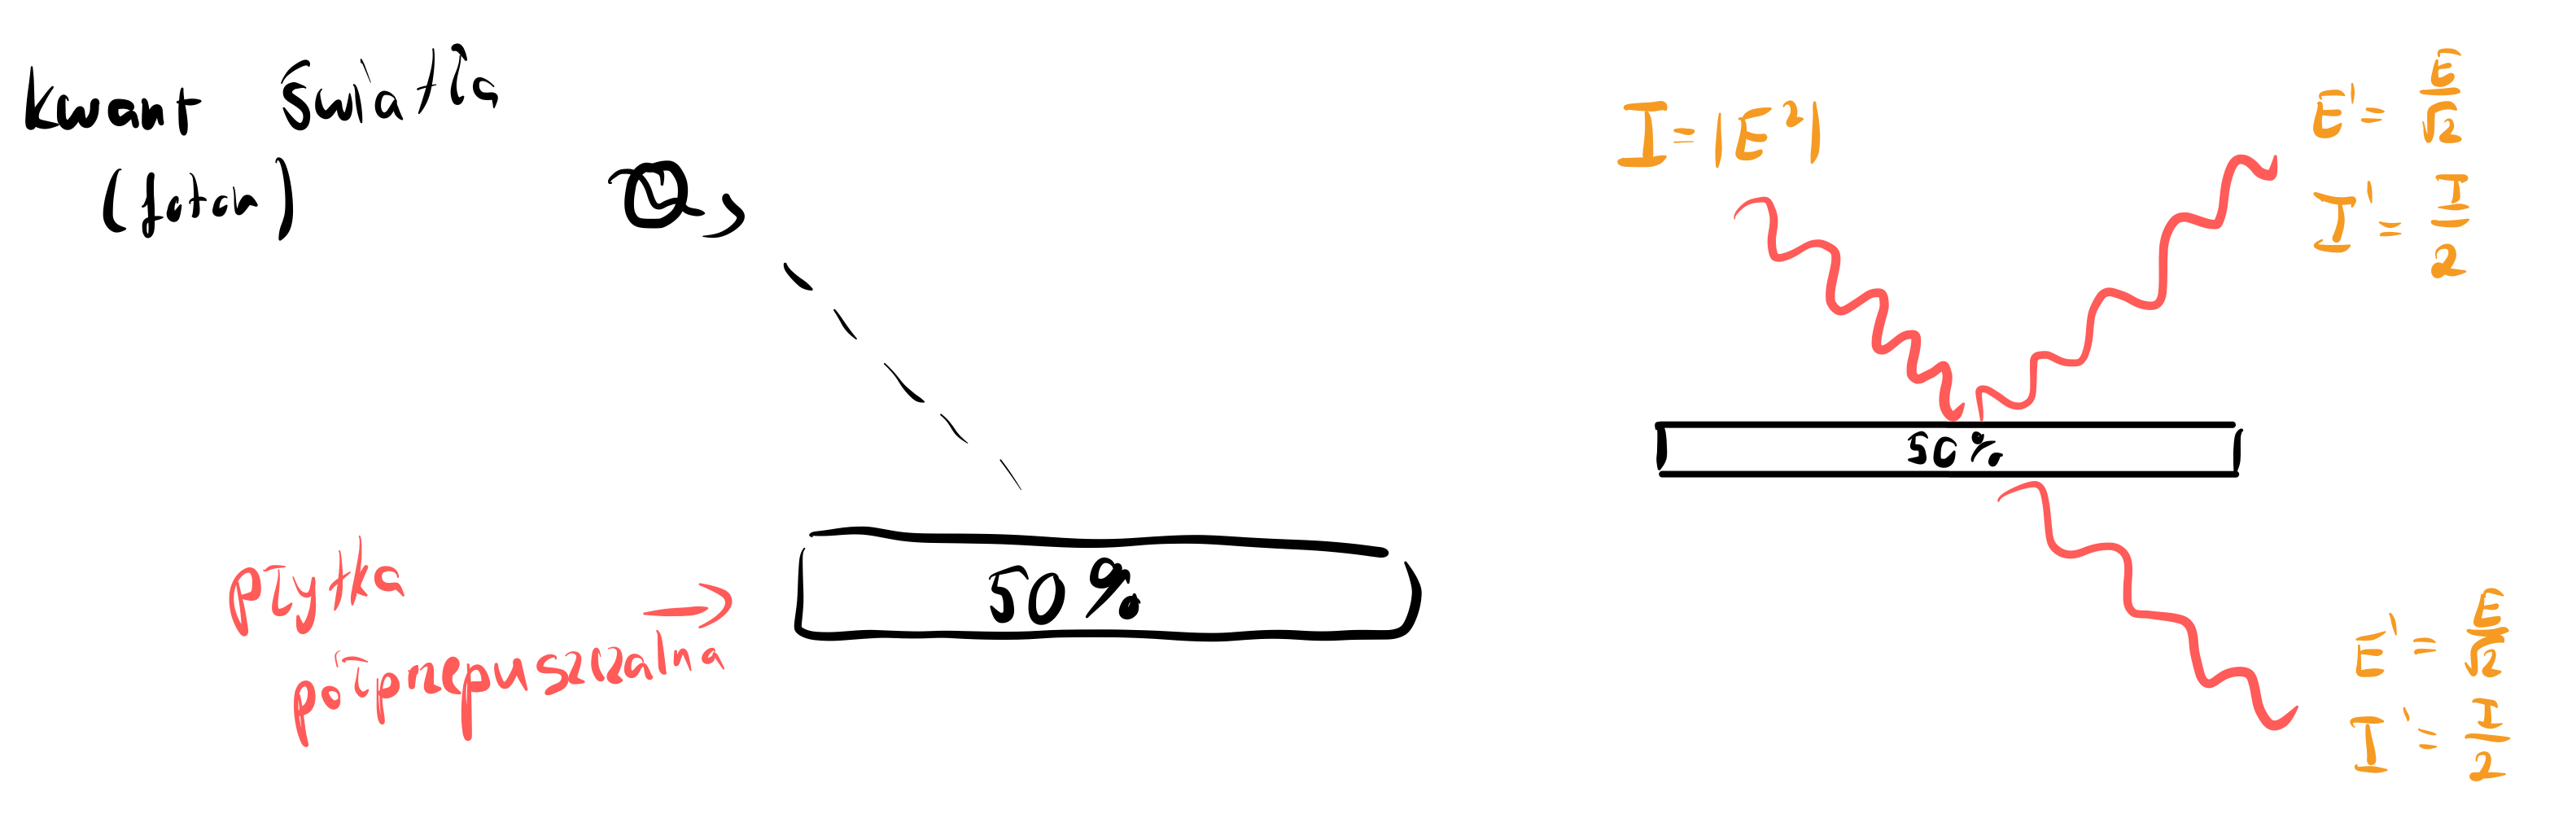
\includegraphics[width=\linewidth]{Wyk_1_Rys_1.jpeg}
        \caption{Demonstracja działania płytki półprzepusczalnej.}
        \label{lec_1:fig:plytka_polprzepuszczalna}
    \end{figure}
    
    \ind{Teoria parametrów ukrytych} - Teoria, że w kwantach energii występują nierejestrowane przez nas parametry, które jednakowoż zawsze determinują rozróżnienie kwantów energii. Parafrazując Drażana, dodawanie fotonom(kwantom) "włosów", "ogonów" itp - elementów rozróżniających je.\\
    
    Jeśli jednak nie chcemy dodawać fotonom 'włosów', ani 'ogonów' i chcielibysmy, żeby wszystkie fotony były "identyczne" to aby odtworzyć zachowanie klasyczne w granicy (podział natężenia 50\%), to musimy uznać, ze foton zachowuje się niedeterministycznie, tj. wprowadzić element probabilistyczny. Wtedy z prawdopodobieństwem 50\% każdy foton przechodzi lub odbija się.
    
    \begin{figure}[!ht]
        \centering
        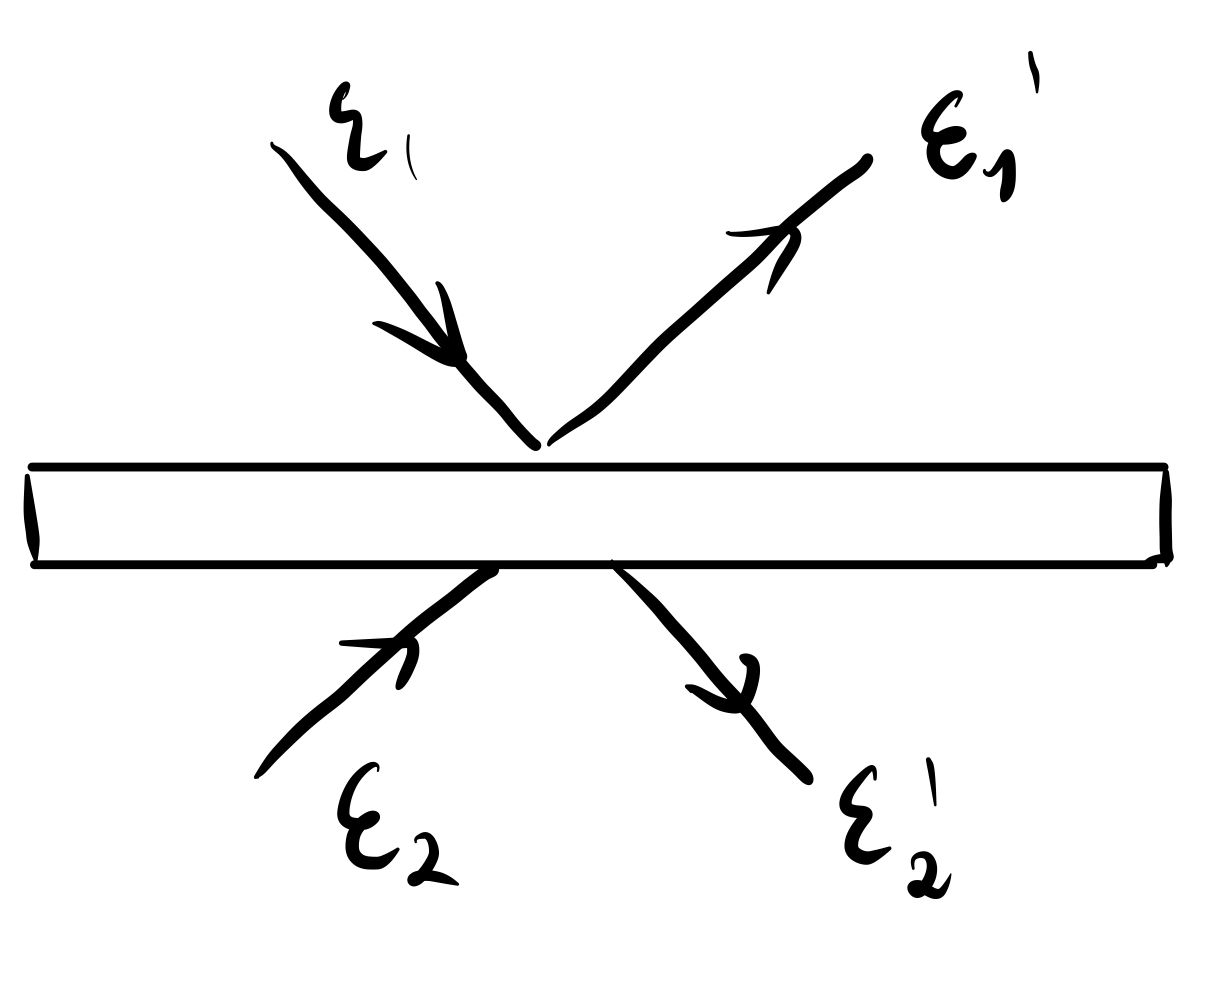
\includegraphics[width=0.6\linewidth]{Wyk_1_Rys_2.jpeg}
        \caption{Demonstracja działania płytki światłodzielącej ({\it Beam Splitter}).}
        \label{fig:lec_1:beam_splitter}
    \end{figure}
    
    Kiedy patrzymy na płytkę światłodzielącą (Rysunek \ref{fig:lec_1:beam_splitter}), to możemy przedstawiać bieg promienia w niej jako superpozycję fal (zapis macierzowy).
    \[\mqty[\E_1' \\ \E_2'] = B \mqty[\E_1 \\ \E_2] \implies \mqty[\R_1 & \T_2 \\ \T_1 & \R_2]\]
    Gdzie $\E_1' = \R1\E_1 + \T_2\E_2$. Chcemy, żeby \emph{energia była zachowana} \[\implies \vqty{\E_1}^2 + \vqty{\E_2}^2 = \vqty{\E_1'}^2 + \vqty{\E_2'}^2\]
    Co możemy też tłumaczyć jako zachowanie długości wektora $ \mqty[\E_1' \\ \E_2']$, czyli macierz $B$ jest macierzą \emph{Unitarną}, tj. $B\cdot B^\dag = 1$. 
    
    \[
        B B^\dag = \mqty[\R_1^\ast & \T_1^\ast \\ 
        \T_2^\ast & \R_2^\ast] 
        \cdot 
        \mqty[\R_1 & \T_2 \\ \T_1 & \R_2] = 
        \mqty[\vqty{\R_1}^2 + \vqty{\T_1}^2 & \R_1^\ast\T_2 + \T_1^\ast R_2 \\ 
        \R_1\T_2^\ast + \T_1 R_2^\ast & \vqty{\R_2}^2 + \vqty{\T_2}^2] = 
        \mqty[1 & 0 \\ 0 & 1]
    \]
    
    Wynika stąd, że $\vqty{\R_1}^2 = \vqty{\R_2}^2 = R$ - współczynnik odbicia natężenia, a $\vqty{\T_1}^2 = \vqty{\T_2}^2 = T$ - współczynnik transmisji natężenia, gdzie $R + T = 1$.
    
    W związku z tym też ogólnie mówiąc np.$ B = \mqty[\sqrt{R} & \sqrt{T} \\ -\sqrt{T} & \sqrt{R}]$, a $B_{50\%} = \frac{1}{2} \mqty[1 & 1 \\ -1 & 1]$. Tj. $B \in \mathcal{U}(2)$
    
    \section{Superpozycja}
    
    Pokażemy zjawisko interferencji w sensie kwantowym patrząc na kanoniczny przykład - \ind{Interferometr Macha-Zehndera}, widoczny na Rysunku \ref{fig:lec_1:interferometer}. Rozpatrujemy od teraz falę padającą postaci $\mqty[\E \\ 0]$.
    
    \begin{figure}[!ht]
        \centering
        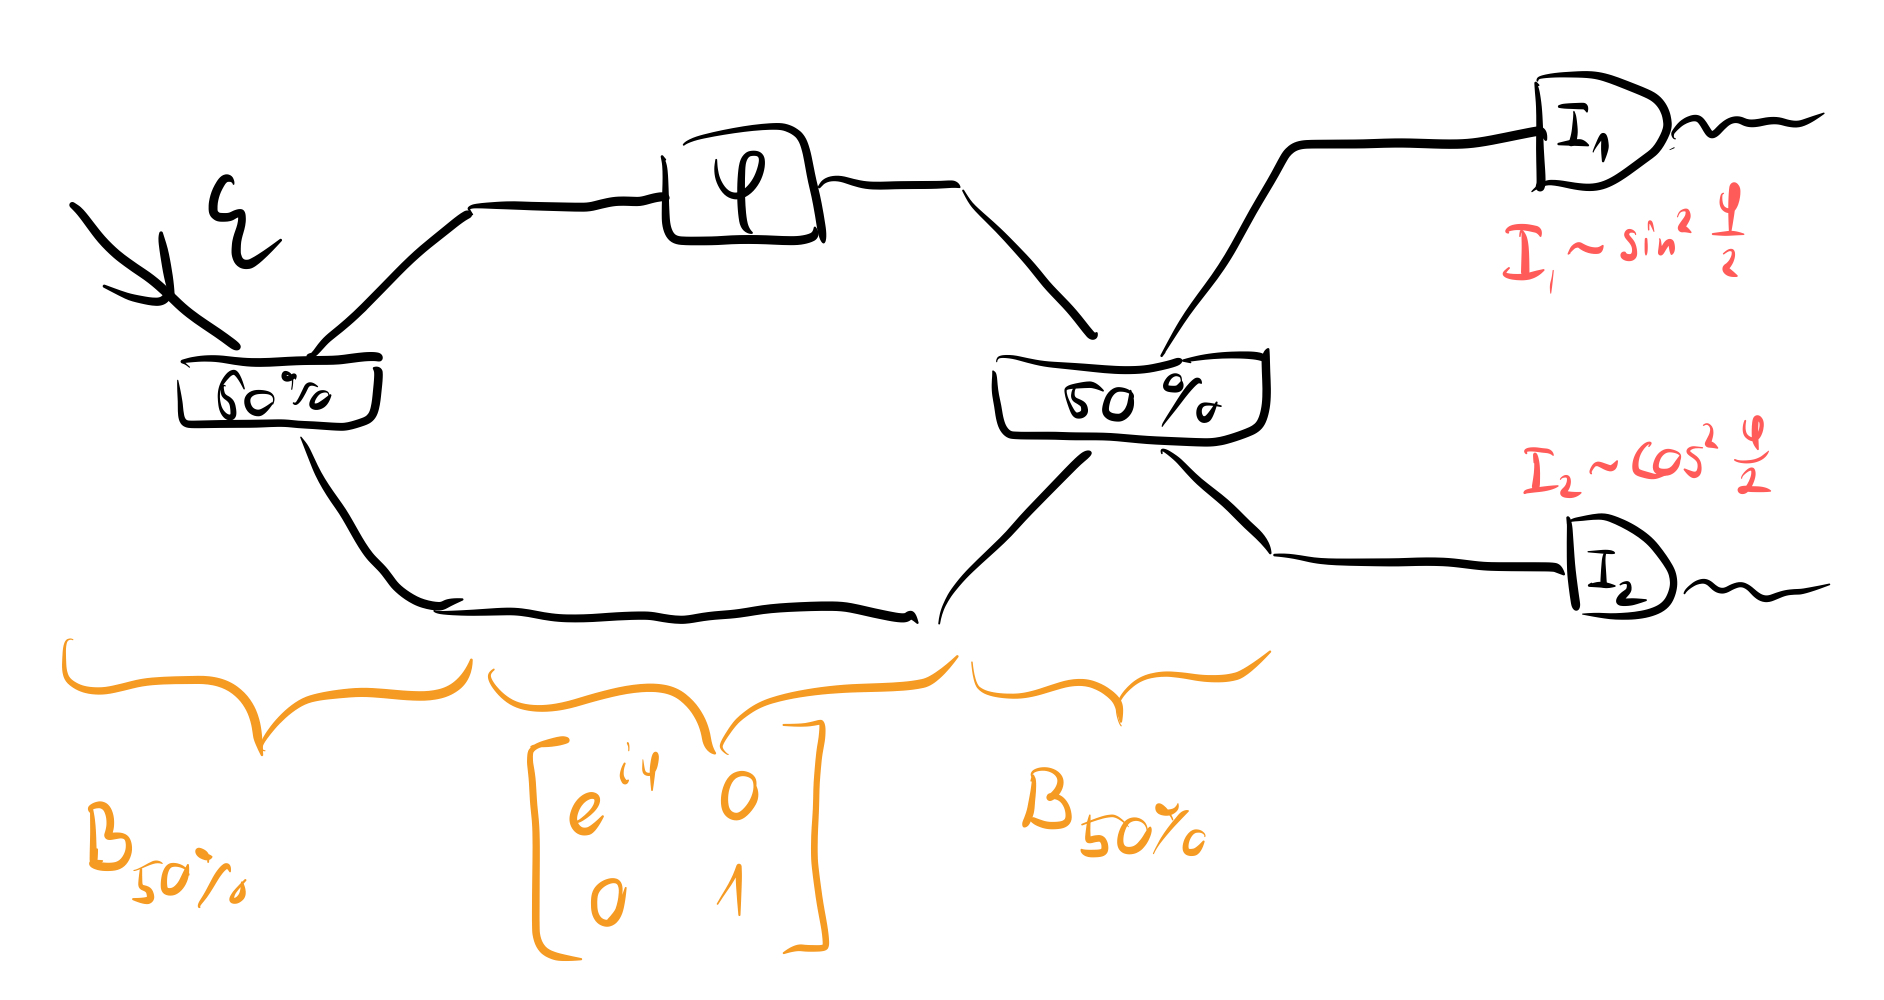
\includegraphics[width=0.8\linewidth]{Wyk_1_Rys_3.jpeg}
        \caption{Schemat konstrukcji Interferometru Macha-Zehndera wraz z podpisem macierzami Jonesa}
        \label{fig:lec_1:interferometer}
    \end{figure}
    
    \begin{figure}[!ht]
        \centering
        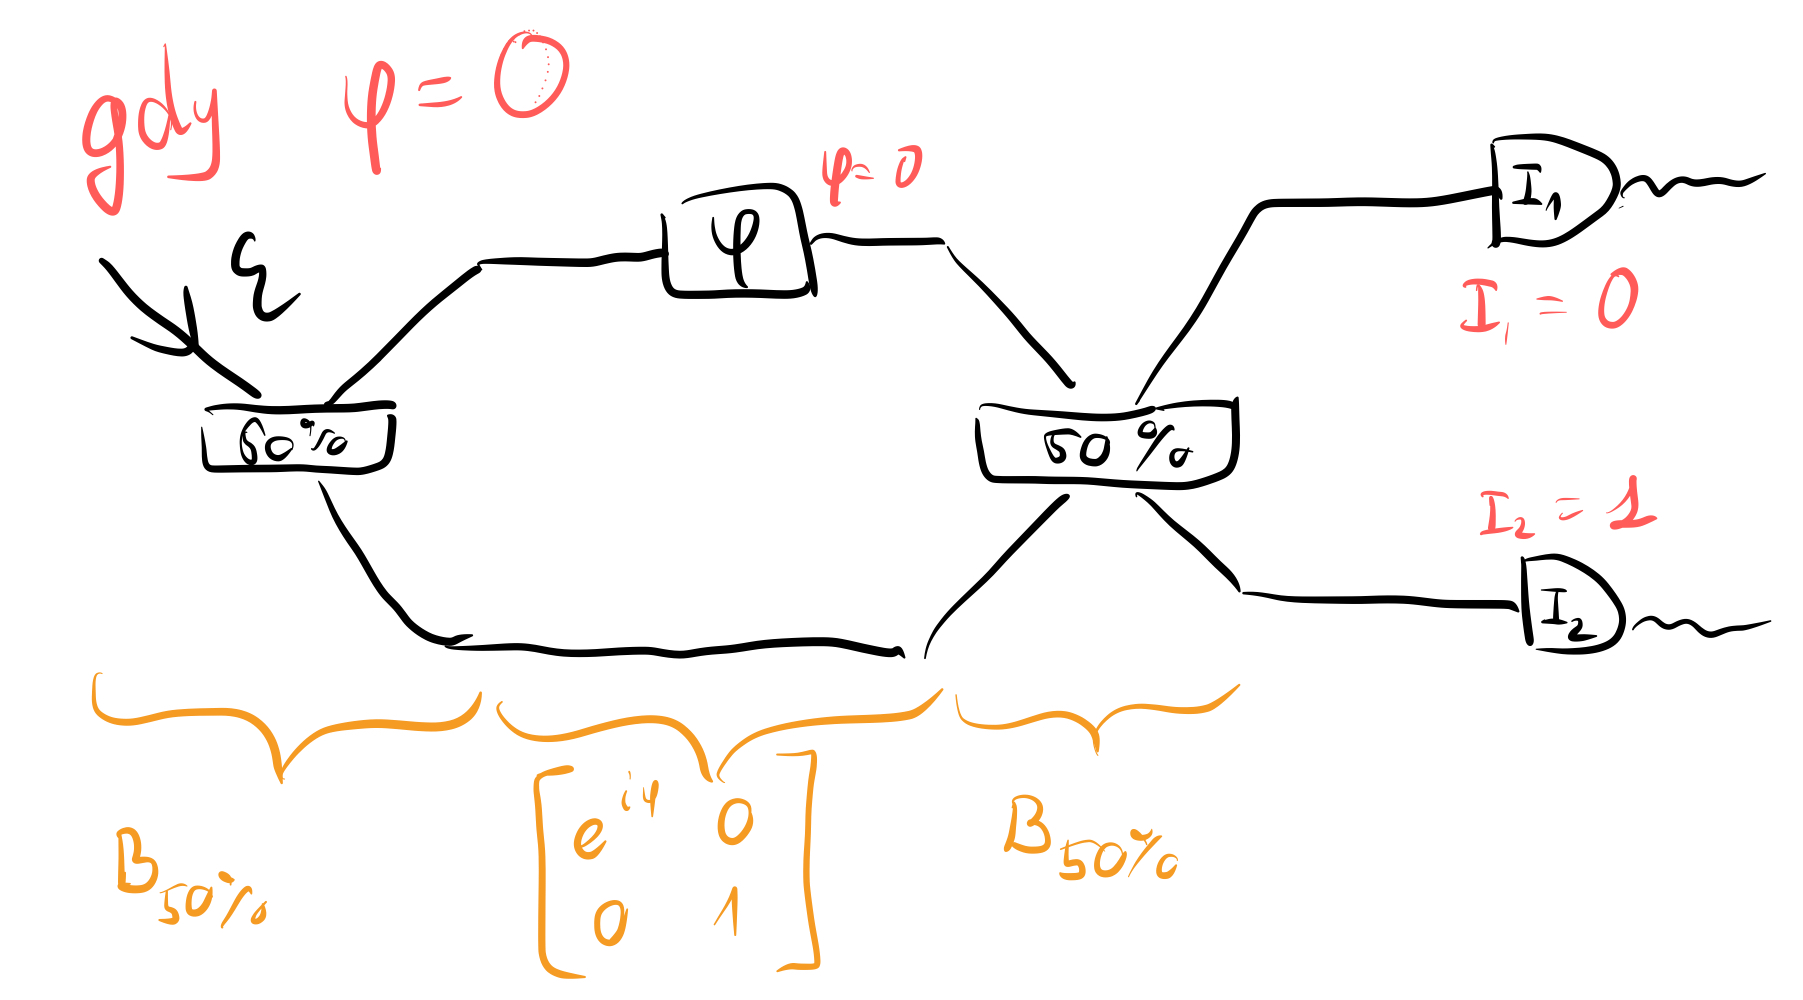
\includegraphics[width=0.8\linewidth]{Wyk_1_Rys_4.jpeg}
        \caption{Schemat konstrukcji Interferometru Macha-Zehndera wraz z podpisem macierzami Jonesa w przypadku zerowej zmiany fazy, tj. w szczególności dla jednego fotonu}
        \label{fig:lec_1:interferometer_phi_0}
    \end{figure}
    
    Teraz aby zrozumieć jak w takim układzie zachowuje się foton musimy odejść od klasycznego myślenia, że leci on jakąś drogą, a musimy przejść do myślenia o jego drodze jako \emph{nieokreślonej}, tj. do momentu wykonania pomiaru (wejścia w interakcję z nim) podąża on jednocześnie wszyskimi możliwymi dla siebie trajektoriami, tym samym przyjmując właściwości falowe. Da to efekt jak ten widoczny na Rysunku \ref{fig:lec_1:interferometer_phi_0}.
    
    Od teraz ten stan 'obierania wszystkich możliwości na raz' przez foton będziemy określać jako \subind{stan fotonu}{Stan!fotonu} oznaczany $\ket{\Psi}$. Tłumaczy się to na funkcję gęstości prawdopodobieństwa znalezienia fotonu w jego możliwych trajektoriach.
    
    W szczególności w opisywanym wyżej przypadku stan $\ket{\Psi}$ będzie opisywany przez \emph{superpozycję} stanów 1 i 2 odpowiadających pójściem drogą odpowiednio górną i dolną, tj. $\ket{\Psi} = \mqty[\Psi_1 \\ \Psi_2]$ gdzie $\Psi_i$ - aplituda prawdopodobieństwa obrania ścieżki $i$, a $p_i = \qty|\Psi_i|^2$ - prawdopodobieństwo, że foton leci i-tą trajektorią.
    
    \begin{equation}
        \ket{\Psi} = \Psi_1\ket{1} \oplus \Psi_2 \ket{2}
        \label{eq:lec_1:superpozycja}
    \end{equation}
    
    Gdzie znakiem $\oplus$ oznaczamy dodawanie fal. Ta operacja to \ind{Superpozycja}. Warto też zanotować, że skoro $\qty|\Psi_i| = p_i$ to ich suma musi się dodawać do 1 
    \[
        \sum_i \qty|\Psi_i|^2 = 1
    \]
    ({\it innymi słowy prawdopodonbieństwo znalezienia fotonu w całej przestrzeni zdarzeń jest 1})
    
    Dla zbudowania intuicji na ten moment możemy sobie utożsamiać tę funkcję pradopodobieństwa z obserwowanym natężeniem światła:
    \[
        \qty|\Psi_i|^2 \sim \qty|\E_i|^2 \sim I_i
    \]
    
\section{Hipoteza De Broigle'a}
{\it Side note 1}: W naszych rozważaniach nie będzie mieć znaczenia faza całkowita, znaczenie będzie mieć tylko faza względna między ramionami, tj. $\E_i \to e^{i \xi} \E_i$. Innymi słowy, 'globalna faza' {\color{brown} nie istnieje!.}

Wyszliśmy w naszych dywagacjach od myślenia o fotonach jako o obiektach falowych, ale nie można zapomnieć o tym, że fotony mają również właściwości korpuskularne, więc sugeruje to, że dla materii też to powinno działać. W związku z tym \ind{Hipoteza De Broigle'a} odpowiadać nam będzie za opisanie 'fal materii', gdzie ich długość fali to będzie:
\[
    \lambda = \frac{h}{p}
\]
Co dla światła ma interpretację:
\[
    p = \frac{E}{c} = \frac{h \cdot \mu}{c} = \frac{h}{\lambda}
\]
Gdzie $E$ - Energia.
    
    Further reading: 
    \begin{itemize}
        \item \link{http://studenci.fuw.edu.pl/~kc427902/Prezentacje_Kwanty/wyklad1-foton.pdf}{Notatki Demko do tego wykładu}
        \item \link{http://studenci.fuw.edu.pl/~kc427902/Prezentacje_Kwanty/cwiczenia1.pdf}{Zadanka na ćwiczenia 1}
        \item \link{http://studenci.fuw.edu.pl/~kc427902/Prezentacje_Kwanty/cwiczenia1.pdf}{Zadanka na ćwiczenia 2}
    \end{itemize}
\end{lecture}

% ------------------------------------------------------------------------
% Wykład 04.03.2022

\begin{lecture}

\section{Stany i pomiary kwantowe}
W tym wykładzie zajmiemy się powoli formalizowaniem intuicji nabywanej na poprzednim wykładzie. Zdefiniujmy $\ket{i}$ - pewne stany rozróżnialne (istnieje pomiar dający róne wyniki dla różnych stanów).

\begin{emph_box}{\subind{Zasada superpozycji}{Zasada!superpozycji}}
\color{orange}
Jeśli $\ket{1}$ i $\ket{2}$ są dopusczalnymi stanami układu, to "$\ket{1}\oplus\ket{2}$"\footnote{rozumiemy to jako "jednocześnie $\ket{1}$ i $\ket{2}$"} też musi być dopuszczalnym stanem układu
\end{emph_box}

Matematyczna struktura odpowiednia dla superpozycji to:
\begin{itemize}
    \item Przestrzeń Hilberta $\HS$ nad $\CS$
    \item $\HS$ - przestrzeń wektorowa nad $\CS$ z iloczynem skalarnym $\braket{\Psi}{\phi}$, $\ket{\Psi} \in \HS$\footnote{wektor reprezentuje stan}, zupełna\footnote{każdy ciąg Cauchy zbiega do elementu $\HS$}
    \item \uwaga{każda skończenie wymiarowa przestrzeń Hilberta (dim $\HS = d$) jest izomorficzna z $\CS^d$}.
\end{itemize}

\subind{Stan Kwantowy}{Stan!kwantowy}:
Niech $\ket{\Psi} \in \HS$, $\braket{\Psi} = 1$. \uwaga{$\ket{\Psi} \phys e^{i \xi} \ket{\Psi} \implies \ket{\Psi} \phys z \cdot \ket{\Psi}$\footnote{Symbol $\phys$ oznacza 'w interpretacji fizycznej ...'}}\\
Stanem kwantowym nazwiemy też promień w przestrzeni Hilberta $\HS$

\ind{Pomiary kwantowe}:
W przestrzeni Hilberta $\HS$ bierzemy sobie wektory $\ket{a_i} \in \HS$, tworzące bazę ortonormalną w $\HS$. Bedzie to zespół rozróżnialnych stanów różniących się pewną obserwowalną wielkością ficzyną $A$. Czyli przyjmujemy:\\
$\ket{a_i}$ - mają dobrze określoną wartośc wielkości fizycznej $A$. Zawsze jak je mierzymy to dostajemy $a_i$.\\
Innymi słowy, jak mamy kilka wielkości fizycznych $A, B, C, \dots$, to w ogólności {\color{red} nie będziemy mogli znaleźć jednej bazy ortonormalnej} $\ket{a_i, b_i, c_i, \dots}$. Jest to esencja mechaniki kwantowej, że różne wialkości fizyczne związane są z różnymi, niekompatybilnymi wobec siebie bazami, które opisują każdą z osobna.\footnote{Czyli pomiar$\neq$zaglądanie do garnka /sprawdzanie stanu który jest zdeterminowany/}

    \begin{figure}[!ht]
        \centering
        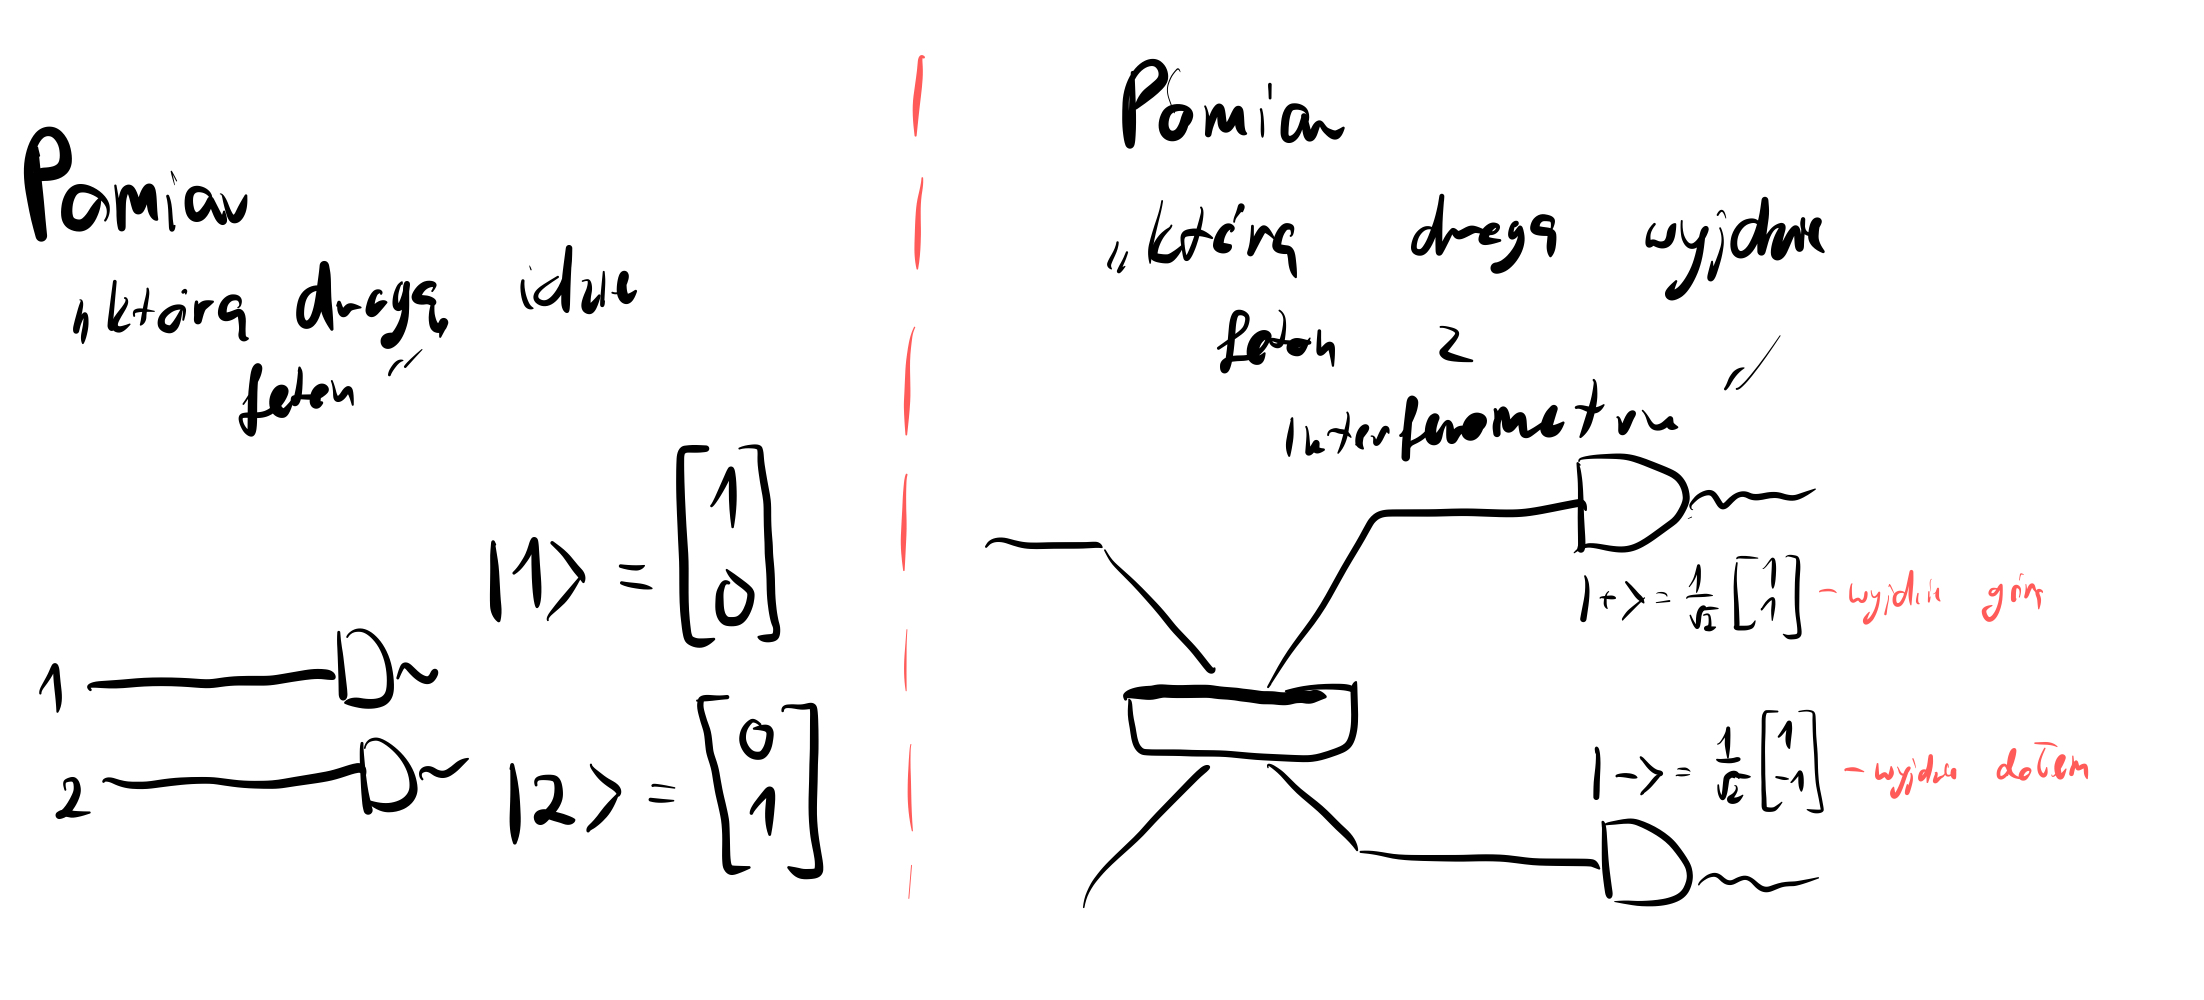
\includegraphics[width=0.8\linewidth]{Wyk_2_Rys_1.jpeg}
        \caption{Porównanie podejść \com{dopracuj opis}}
        \label{fig:lec_2:porownianie}
    \end{figure}
    

\begin{emph_box}{\ind{Postulat pomiarowy}}
    \color{orange} Jeśli $\ket{\Psi}$ jest dowolnym stanem, na którym chcemy zmierzyć wielkość fizyczną $A$, z którą stowarzyszona jest baza $\qty{\ket{a_i}}$. Możemy napisać:
    \[\ket{\Psi} = \sum_i \alpha_i\ket{a_i}\]
    Wtedy uzyskany wynik $a_i$ z prawdopodobieństwem $p_i = \qty|\alpha_i|^2 = \qty|\braket{a_i}{\Psi}|^2$. Tym samym stan po pomiarze ma dobrze określone wielkości $a_i$, tj. jest $\ket{\Psi} = \ket{a_i}$.
\end{emph_box}
 Czyli też jak już raz dokonamy pomiaru na stanie kwantowym to on już nie wróci do możliwości interferencji, i za każdym kolejnym pomiarem już będziemy obserwować ten sam stan, tj. zacznie się zachowywać jakby był klasyczny.
    
\ind{Observabl-a}:
Z pomiarem wielkości A $\qty(\qty{\ket{a_i}})$ stowarzyszamy operator 
\[
    \hat{A} = \sum_i a_i \ketbra{a_i}
\]
gdzie $\hat{A}$ jest operatorem Hermitowskim\footnote{Operator hermitowski - $A^\dagger = A$} czyli w szczególności mając $\hat{A}$ możemy też znaleźć $\qty{\ket{a_i}}$ robiąc rozkład własny.

\begin{align*}
\hline \hline
\end{align*}

{\it Crash course z notacji Diraca:}\\
\textbf{ket}:
\[
    \ket{a} = \mqty[a_1 \\ a_2 \\ \vdots \\ a_n] = \vb{v}
\]
\textbf{bra}:
\[
    \bra{a} = \ket{a}^\dagger = \mqty[a_1, a_2, \cdots, a_n]^\ast = \vb{v}^\dagger
\]
Czyli jak je połączymy dostajemy \textbf{braket}:
\[
    \braket{a}{b} = \mqty[a_1, a_2, \cdots, a_n]^\ast \cdot \mqty[b_1 \\ b_2 \\ \vdots \\ b_n] = \vb{v} \cdot \vb{v}^\ast = liczba\footnote{Iloczyn skalarny}
\]
Zaś z kolei jak pomnożymy w odwrotnej koleności mamy \textbf{ketbra}:
\[
    \ketbra{a}{b} =  \mqty[a_1 \\ a_2 \\ \vdots \\ a_n] \cdot \mqty[a_1, a_2, \cdots, a_n]^\ast = M \in M(\CS)_n^n
\] co rozumiemy też jako operator rzutowy.

\begin{align*}
\hline \hline
\end{align*}

Obserwable jest wygodniej liczyć jako wartości oczekiwane z jakichś rozkłądów prawdopodobieństw:\\
\[
    \expval{A} = \sum_i p_i a_i = \sum_i \qty|\braket{a_i}{\Psi}|^2 \cdot a_i
\]
Gdzie wiemy, że człon $\qty|\braket{a_i}{\Psi}|^2$ możemy rozpisać jako:
\[
    \qty|\braket{a_i}{\Psi}|^2 = \qty|\braket{\Psi}{a_i}|^2 = \braket{\Psi}{a_i}\braket{a_i}{\Psi} = \bra{\Psi} \quad \ketbra{a_i} \quad \ket{\Psi}
\]
W związku z tym możemy dalej rozpisać $\expval{A}$ jako:
\[
    \expval{A} = \bra{\Psi} \quad \sum_i a_i \ketbra{a_i} \quad \ket{\Psi} =\footnote{${\color{blue} \sum_i a_i \ketbra{a_i} = \hat{A}}$} \ev{\hat{A}}{\Psi}
\]


\end{lecture}


\tableofcontents

\listoffigures

\printindex

\end{document}